% Beyond Density Matrices: Geometric Quantum States
% 	formerly:
% What is a Quantum State?
%
% fa: 4/31/20, 5/4/20, 7/15/20
% jpc: 5/1/20, 5/6/20, 7/19/20

%\documentclass[draft,nofootinbib,prl,twocolumn,showpacs,showkeys,groupaddress,preprintnumbers,floatfix]{revtex4-1}
\documentclass[draft,nofootinbib,pre,twocolumn,showpacs,showkeys,preprintnumbers,floatfix]{revtex4-1}

\usepackage{dynlearn}
\usepackage{physics}
\usepackage{multibib}
\newcites{SM}{SM References}
% \usepackage[utf8]{inputenc}
\usepackage{mathrsfs}
\usepackage[english]{babel}
\usepackage{amssymb,amscd}
\newtheorem{theorem}{Theorem}
\newtheorem{hypothesis}{Hypothesis}

% \newcommand{\norm}[1]{\left\Vert#1\right\Vert}
% \newcommand{\abs}[1]{\left\vert#1\right\vert}
% \newcommand{\set}[1]{\left\{#1\right\}}
% \newcommand{\R}{\mathbb{R}}
\newcommand{\e}{\mathrm{e}}
\newcommand{\Hilb}{\mathcal{H}}
\newcommand{\eps}{\varepsilon}
\newcommand{\To}{\longrightarrow}
\newcommand{\BX}{\mathbf{B}(X)}
\newcommand{\A}{\mathcal{A}}
\newcommand{\HH}{\Hilb}
\newcommand{\g}{\mathfrak{g}}
\newcommand{\Ug}{\mathcal{U}\mathfrak{g}}
\newcommand{\Tg}{\mathcal{T}\mathfrak{g}}
\newcommand{\Sg}{\mathcal{S}\mathfrak{g}}
\newcommand{\Us}{\mathcal{U}\mathfrak{s}}
\newcommand{\Ss}{\mathcal{S}\mathfrak{s}}
% \DeclareMathOperator{\Tr}{Tr}
\DeclareMathOperator*{\argmax}{arg\,max}
\DeclareMathOperator*{\argmin}{arg\,min}
\newcommand{\Ut}[1]{\undertilde{#1}}
\newcommand{\1}{\mathbbm{1}}
\newcommand{\circled}[1]{\tikz[baseline=(C.base)]\node[draw,circle,inner sep=1. 2pt,line width=0.2mm,](C) {\small #1};\!}
\newcommand{\Pexp}[1]{\mathrm{Pexp} \left[ #1 \right] }
\newcommand{\Ch}[1]{ \mathrm{Ch} \; #1}
\newcommand{\Sh}[1]{ \mathrm{Sh} \; #1}
% \newcommand{\Ket}[1]{ \left| #1 \right\rangle}
% \newcommand{\Bra}[1]{ \left\langle #1 \right|}
\newcommand{\Scal}[2]{ \left\langle #1 | #2 \right\rangle}
\newcommand{\KetQ}[1]{ \left| #1 \right]}
\newcommand{\BraQ}[1]{ \left[ #1 \right|}
\newcommand{\ScalQ}[2]{ \left[ #1 | #2 \right]}
\newcommand{\Miss}[2]{ \left[ #1 | #2 \right\rangle}
\newcommand{\MissQ}[2]{ \left\langle #1 | #2 \right]}
\newcommand{\ZT}{\undertilde{z}}
\newcommand{\Z}{\zeta}
\newcommand{\MV}[1]{\left\langle #1 \right\rangle}
\newcommand{\MC}[1]{\left\langle #1 \right\rangle_{\mathrm{mc}}}
% \newcommand{\braket}[2]{\langle #1 | #2 \rangle}
% \newcommand{\ketbra}[2]{| #2 \rangle\langle #1 |}
% \newcommand{\ket}[1]{| #1 \rangle}
% \newcommand{\bra}[1]{\langle #1 |}
\renewcommand{\equiv}{\coloneqq}
\newcommand{\PP}[4]{\mathbin{_{#2} P^{#1}_{#3}} \left[ #4 \right]}
\newcommand{\intP}{\int_{\mathcal{P}(\mathcal{H})} \!\!\!\!\!\!\!\!\!}
\newcommand{\intPB}{\int_{\mathcal{P}(\overline{\mathcal{H}})} \!\!\!\!\!\!\!\! \!}
\newcommand{\PH}{\mathcal{P}(\mathcal{H})}

\def\d{\delta}
\def\f{\frac}
\def\om{\omega}
\def\w{\wedge}
\def\la{\langle}
\def\ra{\rangle}
\newcommand{\p}{\partial}
\newcommand{\n}{\nabla}

\newcommand{\cg}[1]{{\color{blue}[[CG: #1]]}}
\newcommand{\fa}[1]{{\color{red}[[FA: #1]]}}
\newcommand{\cut}[1]{{\color{purple}[[CUT?: #1]]}}

\newenvironment{entry}
  {\begin{list}{--}{
      \setlength{\topsep}{0pt}
      \setlength{\itemsep}{0pt}
      \setlength{\parsep}{0pt}
      \setlength{\labelwidth}{5pt}
      \setlength{\itemindent}{0pt}}}{\end{list}}

\def\tbf #1 {\textbf{#1} }

\begin{document}

\def\ourTitle{%
% Interpretation of the Geometric Quantum State
% What is a Quantum State?
A phenomenological theory of information transport
}

\def\ourAbstract{%
TBD
}

\def\ourKeywords{%
Quantum Mechanics, Geometric Quantum Mechanics
}

\hypersetup{
  pdfauthor={Fabio Anza},
  pdftitle={\ourTitle},
  pdfsubject={\ourAbstract},
  pdfkeywords={\ourKeywords},
  pdfproducer={},
  pdfcreator={}
}

%%%%%%%%%%%%%%%%%%%%%%%%%%%%%%%%%%%%%%%%%%%%%%%%%%%%%%%%%%%%%%%%%%%%%%%%%%%%%%%

\title{\ourTitle}

\author{Fabio Anza}
\email{fanza@ucdavis.edu}

%\author{James P. Crutchfield}
%\email{chaos@ucdavis.edu}

\affiliation{Complexity Sciences Center and Physics Department,
University of California at Davis, One Shields Avenue, Davis, CA 95616}

\date{\today}
\bibliographystyle{unsrt}

\begin{abstract}
\ourAbstract
\end{abstract}

\keywords{\ourKeywords}

\pacs{
05.45.-a  %  Nonlinear dynamics and nonlinear dynamical systems
89.75.Kd  %  Complex Systems: Patterns
89.70.+c  %  Information science
05.45.Tp  %  Time series analysis
%02.50.Ey  %  Stochastic processes
%02.50.-r  %  Probability theory, stochastic processes, and statistics
%02.50.Ga  %  Markov processes
%%%%%%%FROM HERE%%%%%%
%05.20.-y  %  Classical statistical mechanics
%02.40.−k %Geometry, differential geometry, and topology
%03.65.−w %Quantum mechanics
%03.67.−a %Quantum information
%05.30.−d %Quantum statistical mechanics
%05.70.−a %Thermodynamics
%%%%%%%TO HERE%%%%%%
}

\preprint{\arxiv{2008.08682}}

\date{\today}
\maketitle

% \tableofcontents

% \setstretch{1.1}

% Collides with table of contents formatting
% \listoffixmes

% {\bf Lead Paragraph:
% }

\paragraph*{Introduction.} Dynamical systems theory describes long-term
recurrent behavior via a system's \emph{attractors}: stable
dynamically-invariant sets. Said simply there are regions of state
space---points, curves, smooth manifolds, or fractals---the system repeatedly
visits. These objects are implicitly determined by the underlying equations of
motion and the probability distributions they support---Sinai-Bowen-Ruelle (SRB)
measures on the system's state space---are interpreted as the analogs of
thermodynamic macrostates \cite{Eckmann1985,Beck93a}. Here lie the foundations
of classical statistical mechanics.

Building on this, the following introduces tools aimed at studying
analogously-important state-space structures for quantum systems. This requires
developing a more fundamental concept of ``state of a quantum system'',
essentially moving beyond the standard notion of density matrices; though they
can be directly recovered. We call these objects the system's \emph{geometric
quantum states} and, paralleling SRB measures, they are specified by a
probability distribution on the space of pure quantum states.

Quantum mechanics is firmly grounded in a vector formalism in which states
$\ket{\psi}$ are elements of a complex Hilbert space $\mathcal{H}$. These are
the system's \emph{pure states}. To account for more general situations, one
employs \emph{density matrices} $\rho$. These are operators in $\mathcal{H}$
that are positive semi-definite $\rho \geq 0$, self-adjoint $\rho
=\rho^\dagger$, and normalized $\Tr \rho = 1$.

The interpretation of a density matrix as a system's \emph{probabilistic state}
is given by \emph{ensemble theory} \cite{Pathria2011,Greiner1995}. Accordingly,
since a density matrix always decomposes into eigenvalues $\lambda_i$ and
eigenvectors $\ket{\lambda_i}$:
\begin{align}
\rho = \sum_i \lambda_i \ket{\lambda_i}\bra{\lambda_i}
  ~,
\label{eq:DiadDecomp}
\end{align}
one interprets $\rho$ as an ensemble of pure states---the eigenvectors---in
which $\lambda_i$ is the probability of an observer interacting with
state $\ket{\lambda_i}$.

However, this interpretation is problematic: It is not unique. One can write
the same $\rho$ using different decompositions, for example in terms of
$\{ \ket{\psi_k}\} \neq \{\ket{\lambda_i}\}$:
\begin{align*}
\rho = \sum_k p_k \ket{\psi_k}\bra{\psi_k}
  ~.
\end{align*}
Given the interpretation, all the decompositions identify the same quantum
state $\rho$. While one often prefers Eq. (\ref{eq:DiadDecomp})'s diagonal
decomposition in terms of eigenvalues and eigenvectors, it is not the only one
possible. More tellingly, in principle, there is no experimental reason to
prefer it to others. This fact is often addressed by declaring density matrices 
with the same \emph{barycenter} equal. A familiar example of this degeneracy 
is that the maximally mixed state ($\rho \propto \mathbb{I}$) has an infinite 
number of identical decompositions, each possibly representing a physically-distinct 
ensemble.

Moreover, it is rather straightforward to imagine systems that, despite being
in obviously different physical situations, are described by the same density
matrix. For example, consider two distinct state-preparation protocols. In one
case, we prepare $\{\ket{0},\ket{1}\}$ with classical probabilities $p_{0/1} = \frac{1\pm \lambda}{2}$; 
in the other, we prepare states 
\begin{subequations}
\begin{align}
&\ket{\psi_0} = \sqrt{\frac{1+\lambda}{2}} \ket{0} + \sqrt{\frac{1-\lambda}{2}} e^{i\chi}\ket{1}~,\\
&\ket{\psi_1} = \sqrt{\frac{1+\lambda}{2}} \ket{0} + \sqrt{\frac{1-\lambda}{2}} e^{i(\chi + \pi)}\ket{1}~,
\end{align}
\end{subequations}
each with probability $1/2$. It is easy to check that they are described by 
the same $\rho$. It is also easy to see that the two state-preparation protocols
simply traded a classical source of randomness, the bias $p_0 - p_1 = \lambda$, 
for one of quantum nature, the bias $\left\vert \braket{\psi_0}{\psi_1} \right\vert^2 = \lambda$.

The following argues that an alternative---the \emph{geometric
formalism}---together with an appropriately adapted measure theory 
allows to overcome these ambiguities.


%A complete and unambiguous mathematical concept of state should not conflate
%such distinct physical configurations. Not only do such ambiguities lead to
%misapprehending fundamental mechanisms, they also lead one to ascribe
%complexity or randomness where there is none \cite{Ven20}. 

%The following argues that an alternative---the \emph{geometric
%formalism}---together with an appropriately adapted measure theory cleanly
%separates the primary concept of a \emph{system state} from the derived concept
%of a density matrix as the set of all \emph{positive operator-valued
%measurement statistics} a system generates, resolving these ambiguities.

With this perspective in mind, first, we recall the basics of \emph{geometric quantum
mechanics} (GQM). Second, we discuss how it relates to density matrices. Then, we 
analyze two broad settings in which the geometric approach arises naturally.
We consider a quantum system with finite-dimensional Hilbert space, interacting with
another one with (1) infinite-dimensional Hilbert space and (2) finite-dimensional
Hilbert space. These are relevant, respectively, for the contexts of quantum state 
manipulation \cite{Anza20c} and quantum thermodynamics \cite{Anza20b}. After 
discussing the results, we draw out several consequences.

\paragraph*{Geometric quantum mechanics.}
\label{sec:GQM}
References
\cite{STROCCHI1966,Miel68,Kibble1979,Heslot1985,Page87,And90,Gibbons1992,Ashtekar1995,Ashtekar1999,Brody2001,Bengtsson2017,Carinena2007,Chruscinski2006,Marmo2010,Avron2020,Pastorello2015,Pastorello2015a,Pastorello2016,Clemente-Gallardo2013}
give a comprehensive introduction to GQM. Here, we briefly summarize only the
elements we need, working with Hilbert spaces $\mathcal{H}$ of finite dimension $D$.

Pure states are points in the complex projective manifold $\mathcal{P}\left(
\mathcal{H} \right)=\mathbb{C}\mathrm{P}^{D-1}$. Therefore, given an arbitrary
basis $\left\{\ket{e_\alpha} \right\}_{\alpha=0}^{D-1}$, a pure state is
parametrized by $D$ complex homogeneous coordinates $Z = \left\{      Z^\alpha\right\}$, up to
normalization and an overall phase:
\begin{align*}
\ket{\psi} = \sum_{\alpha=0}^{D-1} Z^\alpha \ket{e_\alpha}
  ~,
\end{align*}
where $Z \in \mathbb{C}^{D}$, $Z \sim \lambda Z$, and $\lambda \in
\mathbb{C}/\left\{ 0\right\}$. If the system consists of a single qubit, for
example, one can always use probability-phase coordinates $Z = (\sqrt{1-p},\sqrt{p} e^{i\nu})$.

An \emph{observable} is a function $\mathcal{O}(Z) \in
\mathbb{R}$ that associates to each point  $Z \in \mathcal{P}(\mathcal{H})$ the
expectation value $\bra{\psi} \mathcal{O} \ket{\psi}/\braket{\psi}{\psi}$ of the corresponding
operator $\mathcal{O}$ on state $\ket{\psi}$ with coordinates $Z$:
\begin{align}
\mathcal{O}(Z) = \frac{\sum_{\alpha,\beta} \mathcal{O}_{\alpha,\beta}Z^\alpha \overline{Z}^\beta}{\sum_{\gamma} \left\vert Z^\gamma\right\vert^2}
  ~,
\label{eq:GQM_Observable}
\end{align}
where $\mathcal{O}_{\alpha \beta}$ is Hermitian $\mathcal{O}_{\beta,\alpha} = \overline{\mathcal{O}}_{\alpha,\beta}$.

Measurement outcome probabilities are determined by \emph{positive
operator-valued measurements} (POVMs) $\left\{E_j\right\}_{j=1}^n$ applied to a
state \cite{Nielsen2010,Heinosaari2012}. They are nonnegative operators
$E_j\geq 0$, called \emph{effects}, that sum up to the identity: $\sum_{j=1}^n
E_j = \mathbb{I}$. In GQM they consist of nonnegative real functions $E_j(Z)\ge
0$ on $\mathcal{P}(\mathcal{H})$ whose sum is always unity:
\begin{align}
E_j(Z) = \frac{\sum_{\alpha,\beta}
  \left(E_j\right)_{\alpha,\beta} Z^\alpha \overline{Z}^\beta}{\sum_{\gamma} \left\vert Z^\gamma \right\vert^2}
  ~,
\label{eq:GQM_POVMs}
\end{align}
where $\sum_{j=1}^{n}E_j(Z) = 1$.

The projective Hilbert space of the pure states of a quantum system $\mathcal{P}(\mathcal{H})$ has a preferred
metric $g_{FS}$---the \emph{Fubini-Study metric} \cite{Bengtsson2017}---and an
associated volume element $dV_{FS}$ that is coordinate-independent and
invariant under unitary transformations. The geometric derivation of $dV_{FS}$
is beyond our immediate goals here. That said, it is sufficient to give its
explicit form in the probability-phase coordinate system $Z^{\alpha} =
\sqrt{p_\alpha}e^{i\nu_\alpha}$ that we use for explicit calculations: 
\begin{align*}
dV_{FS}
  & = \sqrt{\det g_{FS}}
  \prod_{\alpha=0}^{D-1} dZ^\alpha d\overline{Z}^\alpha \\
  & =  \prod_{\alpha=1}^{D-1} \frac{dp_\alpha d\nu_\alpha}{2}
  ~.
\end{align*}
Notice how $p_0$ and $\nu_0$ are not involved. This is due to
$\mathcal{P}(\mathcal{H})$'s projective nature which guarantees that we can
choose a coordinate patch in which $p_0 = 1 - \sum_{\alpha=1}^{D-1}p_\alpha$
and $\nu_0 = 0$.

\paragraph*{Geometric quantum states.}
This framework makes it very natural to view a quantum state as a functional
encoding that associates expectation values to observables, paralleling the
$C^{*}$-algebra formulation of quantum mechanics \cite{Strocchi2008a}. 
The idea is that one considers probability density functions on $\mathcal{P}(\mathcal{H})$ (as $q(Z)$),
together with observable functions (as $\mathcal{O}(Z)$). This was introduced 
in Ref. \cite{Brody2001} and here we give a quick summary.

States are functionals $P[\mathcal{O}]$ from the algebra of
observables $\mathcal{A}$ to the real line: 
\begin{align}
P_q[\mathcal{O}]
  = \int_{\mathcal{P}(\mathcal{H})} q(Z) \mathcal{O}(Z) dV_{FS}
  ~,
\label{eq:gqs}
\end{align}
where $\mathcal{O} \in \mathcal{A}$, $q(Z) \geq 0$ is the
normalized distribution associated with functional $P$:
\begin{align*}
P_q[\mathbb{I}] = \int_{\mathcal{P}(\mathcal{H})}
  q(Z) dV_{FS}  = 1
  ~,
\end{align*}
and $P_q[\mathcal{O}] \in \mathbb{R}$. 
In this way, pure states $\ket{\psi_0}$ are functionals with a Dirac-delta
distribution $p_0(Z) = \widetilde{\delta}\left[ Z - Z_0\right]$:
\begin{align*}
P_{0}[\mathcal{O}] &= \intP \widetilde{\delta}(Z-Z_0)\mathcal{O}(Z) dV_{FS} \\
  & = \mathcal{O}(Z_0)  = \bra{\psi_0}\mathcal{O}\ket{\psi_0}
  ~.
\end{align*}
$\widetilde{\delta}(Z-Z_0)$ is shorthand for a coordinate-covariant Dirac-delta in
arbitrary coordinates. In homogeneous coordinates this reads:
\begin{align*}
\widetilde{\delta}(Z - Z_0) \coloneqq \frac{1}{\sqrt{\det g_{FS}}}
  \prod_{\alpha=0}^{D-1} \delta(X^\alpha - X^\alpha_0)
  \delta(Y^\alpha - Y^\alpha_0)
  ~,
\end{align*}
where $Z^\alpha = X^\alpha + iY^\alpha$. In $(p_\alpha,\nu_\alpha)$ coordinates
this becomes simply:
\begin{align*}
\widetilde{\delta}(Z - Z_0) = \prod_{\alpha=1}^{D-1} 2\delta(p_\alpha - p_\alpha^0) \delta(\nu_\alpha - \nu_\alpha^0)
  ~,
\end{align*}
where the coordinate-invariant nature of the functionals $P_q[\mathcal{O}]$ is
now apparent.

In this way, too, mixed states:
\begin{align*}
\rho = \sum_{j}\lambda_j \ket{\lambda_j}\bra{\lambda_j}
\end{align*}
are convex combinations of these Dirac-delta functionals:
\begin{align*}
q_{\mathrm{mix}}(Z) = \sum_{j}\lambda_j \widetilde{\delta}(Z-Z_j)
  ~. 
\end{align*}
Thus, expressed as functionals from observables to the real line, mixed states
are:
\begin{align}
P_{\mathrm{mix}}\left[ \mathcal{O}\right]
  & = \sum_{j} \lambda_j \bra{\lambda_j}\mathcal{O}\ket{\lambda_j}
  ~.
\label{eq:Functional}
\end{align}

Equipped with this tools, one identifies the distribution $q(Z)$ of Eq.
(\ref{eq:gqs}) as a system's \emph{geometric quantum state}. This is a
generalized notion of quantum state.

A simple example of a geometric quantum state is the 
\emph{geometric canonical ensemble}:
\begin{align*}
q(Z) = \frac{1}{Q_\beta} e^{-\beta h(Z)}
  ~,
\end{align*}
where:
\begin{align*}
  Q_\beta & = \int dV_{FS} e^{-\beta h(Z)} ~, \\
  h(Z) & = \bra{\psi(Z)}H\ket{\psi(Z)} ~,
\end{align*}
and $H$ is the system's Hamiltonian operator. This was introduced in 
Refs. \cite{Brody1998}. References \cite{Brody2016} and \cite{Anza20b} 
investigated its potential role in establishing a quantum foundation of
thermodynamics that is an alternative to that based on Gibbs ensembles and von
Neumann entropy. 

\paragraph*{Density matrix.}
The connection between geometric quantum states and density matrices is
two-fold. On the one hand, when $q(Z)$ falls into one of the
two aforementioned cases---Dirac-deltas or finite convex combinations of
them---the present formalism is equivalent to the standard one. However, not
all functionals fall into the Dirac-delta form. Given this, $q(Z)$ is clearly a
more general notion of a quantum system's state than density matrices.

On the other hand, given an arbitrary $q(Z)$, there is a unique
density matrix $\rho^{q}$ associated to $q$:
\begin{align}
\rho^q_{\alpha \beta} & = P_q[Z^\alpha \overline{Z}^\beta] \nonumber \\
  & = \intP dV_{FS} \, q(Z)  \, Z^\alpha \overline{Z}^\beta
  ~.
\label{eq:densitymatrix}
\end{align}
Owing to the specific form of POVMs on $\mathcal{P}(\mathcal{H})$, recall Eq. (\ref{eq:GQM_POVMs}), they
are sensitive to $q(Z)$ only via $\rho^q$. Therefore, if two geometric quantum states 
$q_1$ and $q_2$ induce the same density matrix $\rho^{q_1} = \rho^{q_2}$, then all POVMs
produce the same outcomes.

A well-known consequence of this fact is that two density matrices with the
same barycenter are considered equal, even if they describe experiments with
different physical configurations. In these cases, the statistics of POVM
outcomes are described by the same density matrix. Note that this statement
does not mean that the two physical configurations are the same. Rather, it
means that there is no POVM on the system that distinguishes between $q_1$ and
$q_2$.

To emphasize, consider the example of two geometric quantum states, $q_1$ and
$q_2$, with very different characteristics:
\begin{align*}
q_1(Z) & = 0.864~\tilde{\delta}(Z - Z_{+}) + 0.136~\tilde{\delta}(Z - Z_{-})~,\\
q_2(Z) & = \frac{1}{Q} e^{-\frac{1}{2} \overline{Z}\rho^{-1}Z } 
  ~,
\end{align*}
where $Q = \int_{\mathbb{C}P^1} dV_{FS} e^{-\frac{1}{2}Z \rho^{-1}
\overline{Z}}$, $Z_+ = (0.657,0.418 + i 0.627)$, and $Z_- =
(0.754,-0.364-i0.546)$. However, states $q_1$ and $q_2$ have same density
matrix $\rho$ ($\rho_{00} = 0.45 = 1- \rho_{11}$ and $\rho_{01} = 0.2 - i 0.3
= \rho_{10}^{*}$) and so the same POVM outcomes. From Fig. \ref{fig:Example}
one appreciates the profound difference between $q_1$ and $q_2$, despite the
equality of their POVM statistics.

\begin{figure}[h]
\centering
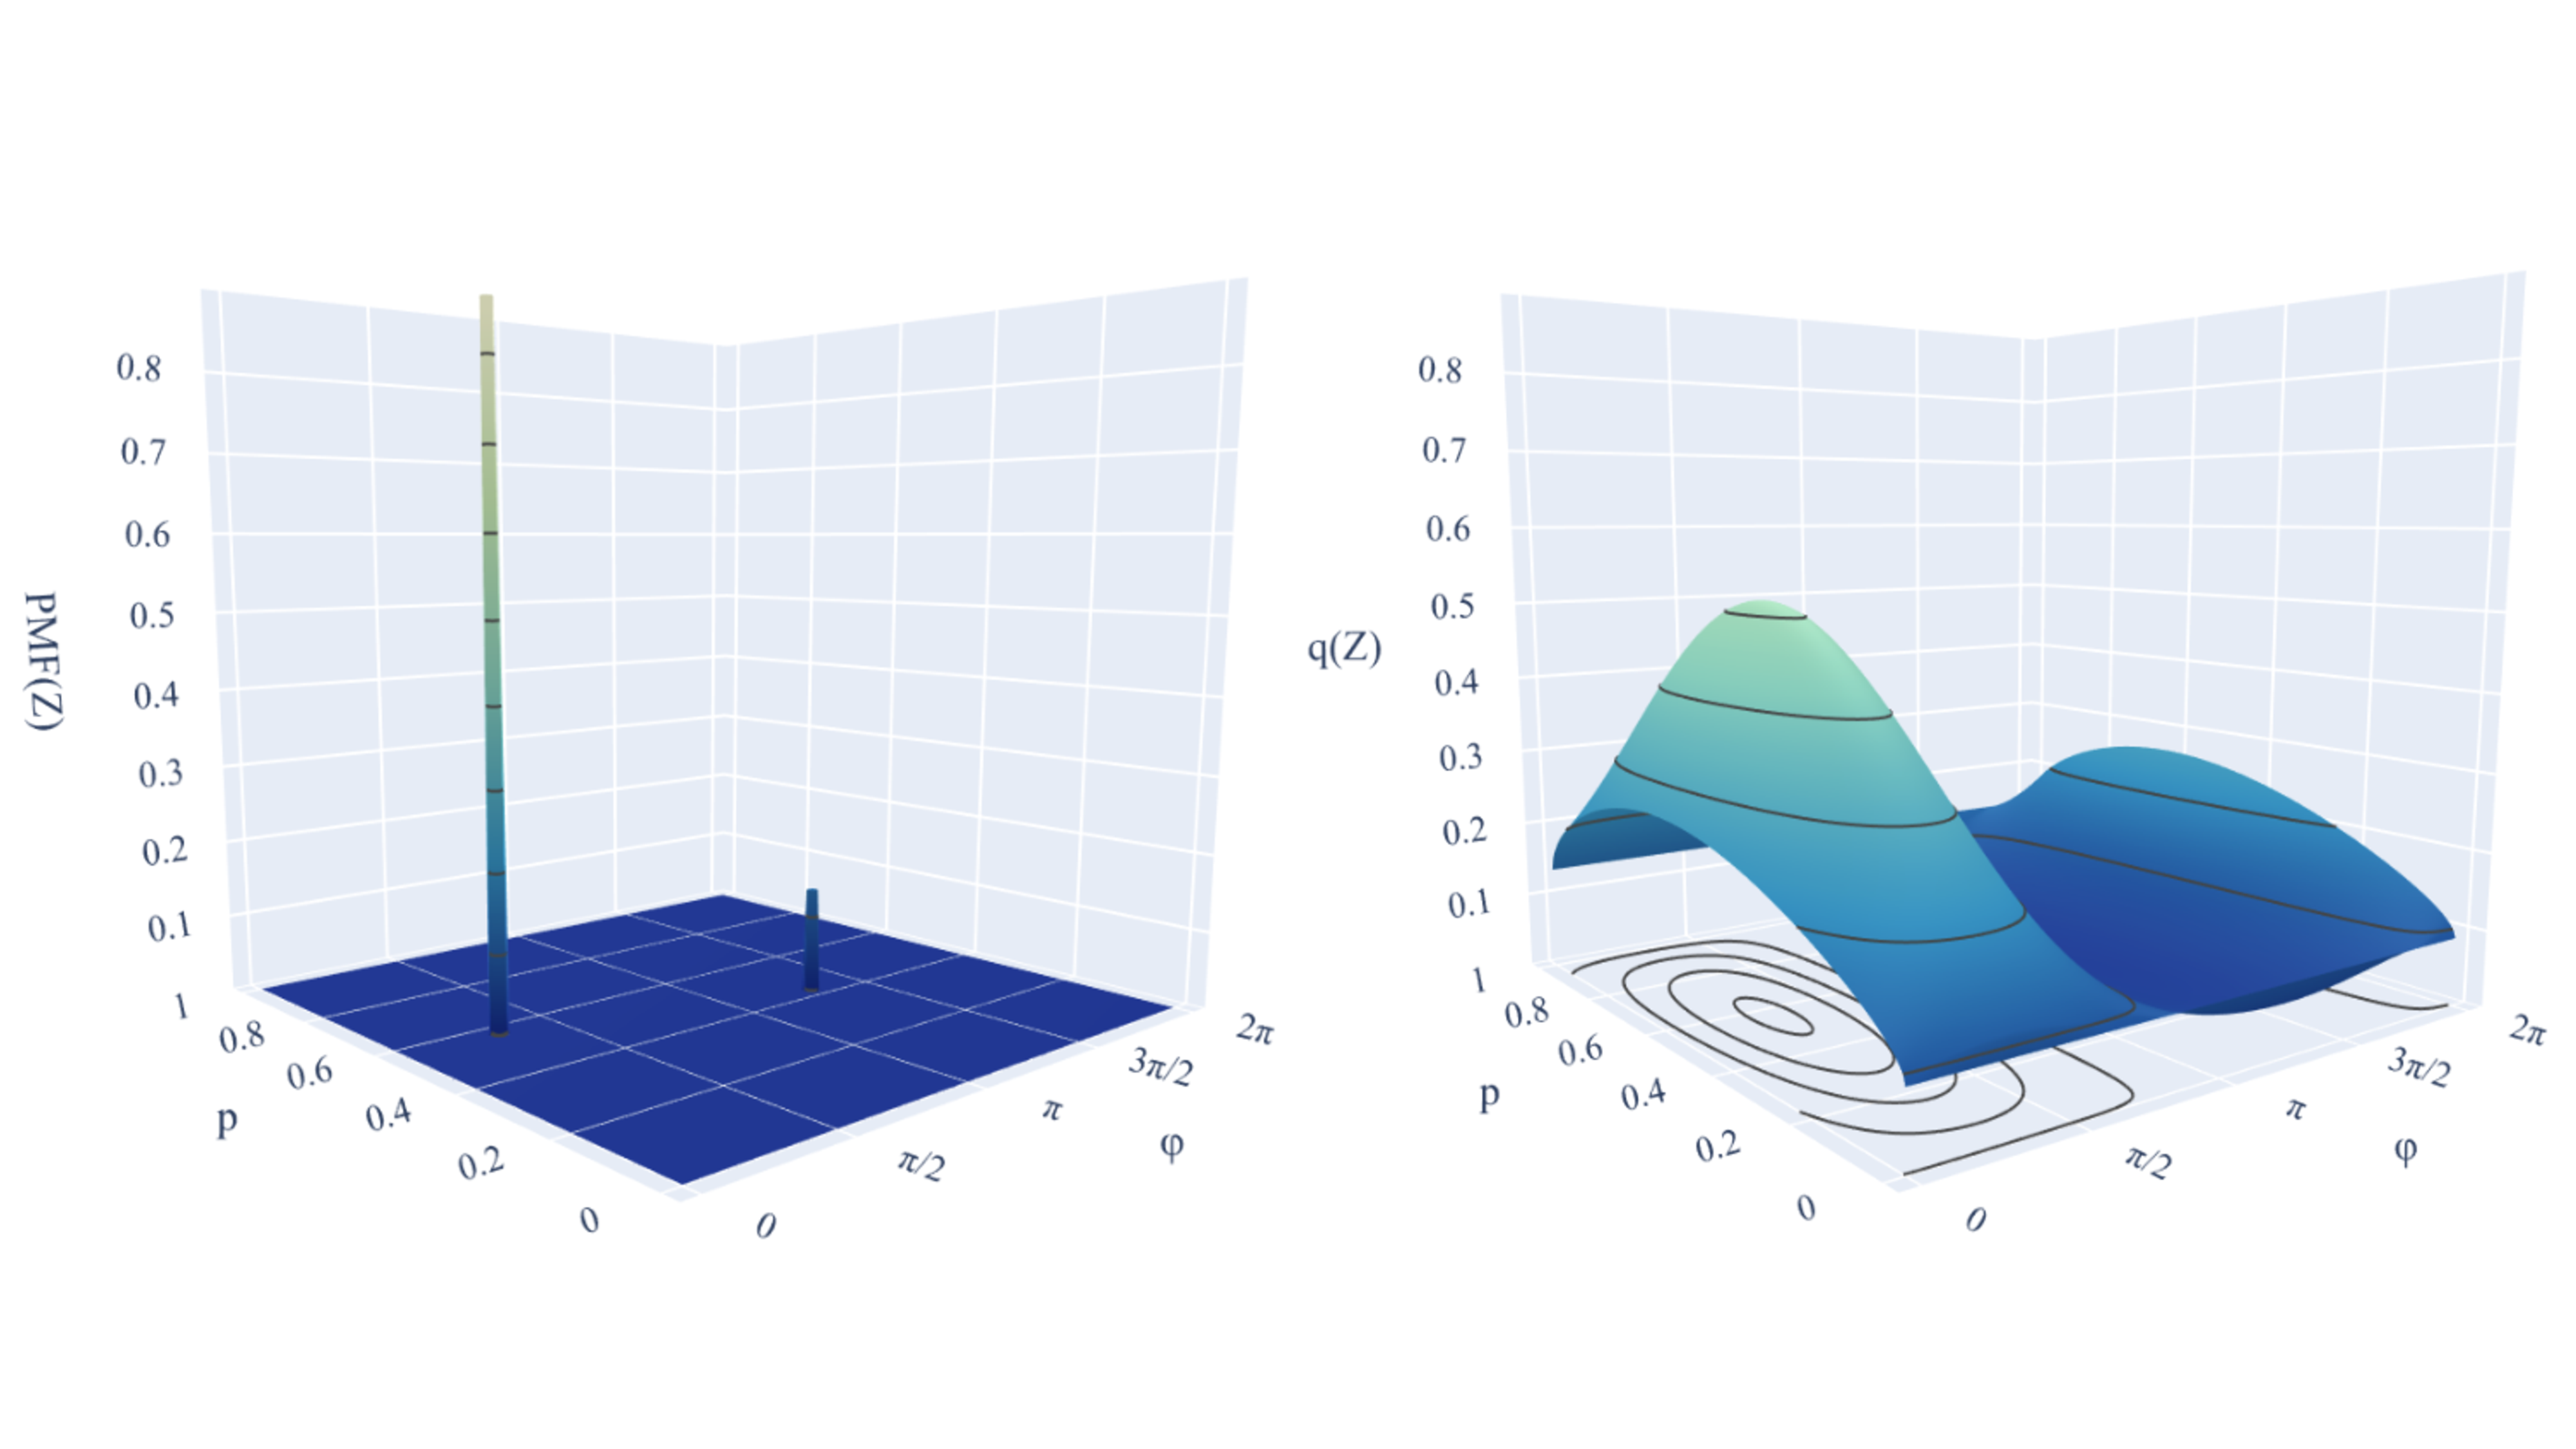
\includegraphics[width=\columnwidth]{img/New_Example.pdf}
\caption{Geometric quantum states in \emph{(probability,phase)} coordinates
	$(p,\phi)$ of $\mathbb{C}P^1$: (Left) Geometric quantum state $q_1$ is the
	convex sum of two Dirac delta-functions, centered on the eigenvectors
	$(p_+,\phi_+) = (0.568,0.983) $ and $(p_-, \phi_-) = (0.432,4.124)$ of
	density matrix $\rho$. (Right) Geometric quantum state $q_2$ differs
	markedly: A smooth distribution across the entire pure-state manifold
	$\mathbb{C}P^1$. However, $q_1$ and $q_2$ have the same density matrix
	$\rho_{q_1} = \rho_{q_2} = \rho$, where $\rho_{00} = 1- \rho_{11} = 0.45$,
	$\rho_{01} = \rho_{10}^{*} = 0.2 - 0.3 i$. $\rho_{\pm}$ are the eigenvalues
	of the density matrix: $\rho_+ = 0.864$ and $\rho_{-}=0.136$. Thus, the
	marked difference in the structure of geometric quantum states $q_1$ and
	$q_2$ is not reflected in their shared density-matrix $\rho_1 = \rho_2 =
	\rho$.
	}
\label{fig:Example} 
\end{figure}

This is particularly important for quantum information processing where one
encounters long-range and long-lived correlational and mechanistic demands.
Quantum computing immediately comes to mind. There, one is not only interested
in measurement outcomes, but also in predicting and understanding how a quantum
system evolves under repeated external manipulations imposed by complex control
protocols.

%In such settings, understanding whether a
%state-preparation protocol produces Dirac-delta-like distributions of pure
%states or more general distributions is paramount to properly address
%computational errors and to analyzing the thermodynamic costs of quantum
%computation.

\paragraph*{State manipulation.}
The following shows that the geometric formalism arises quite naturally when a
discrete quantum system interacts and develops entanglement with a continuous
one. Imagine a protocol controlling a system's continuous degrees of freedom to
manipulate discrete ones that store a computation's result. As a physical
reference, consider quantum particles with a given number of discrete degrees
of freedom (e.g., spin), confined to a region $\mathcal{R} \subseteq
\mathbb{R}^3$. The results we derive do not depend on this choice, since the
technical methods straightforwardly extend to other systems where continuous
and discrete degrees of freedom are mixed. A helpful illustration is
intra-particle entanglement \cite{Pasini2020} that couples position and spin
degrees of freedom to create entangled states. In this way, one manipulates the
spin by only acting on the positional degrees of freedom, possibly via a
potential.

Consider a hybrid quantum system comprised of $N$ continuous degrees of freedom
and $M$ q-dits that are discrete. The entire system's Hilbert space is:
\begin{align*}
\mathcal{H} = \mathcal{H}^c_N \otimes \mathcal{H}^d_M
  ~,
\end{align*}
where $\mathcal{H}_N^c \coloneqq \mathcal{H}_c^{\otimes N}$ hosts $N$ one-dimensional continuous degrees of freedom
and has infinite dimension, while $\mathcal{H}^d_M \coloneqq \mathcal{H}_d^{\otimes M}$ hosts 
$M$ discrete degrees of freedom, each with dimension $d$, and therefore has dimension $d^M$. 
A basis for $\mathcal{H}_N^c$ is provided
by $\left\{\ket{\vec{x}}\right\}$, where $\vec{x} \in \mathcal{R} \subseteq
\mathbb{R}^N$ and a basis for $\mathcal{H}_M^d$ is
$\left\{\ket{s}\right\}_{s=0}^{d^M-1}$. Thus, a generic pure state is:
\begin{align*}
\ket{\psi} = \int_{\mathcal{R}} d\vec{x} \sum_{s} \psi_s(\vec{x})\ket{\vec{x}} \ket{s}
  ~,
\end{align*}
where $\vec{x}$ is a dimensionless counterpart of the physical continuous
degrees of freedom, achieved by multiplying its value by appropriate physical
quantities. So, the measure $d\vec{x}$ has no physical dimension. For an
electron in a box, for example, this is achieved by renormalizing with the box's
total volume.

The following theorem establishes that this can be done constructively.

\begin{theorem}
\label{MainTheo}
Any $\ket{\psi} \in \mathcal{H}$ can be written as:
\begin{align}
\ket{\psi} = \int_{\mathcal{R}}d\vec{x} f(\vec{x}) \ket{x}\ket{q(\vec{x})} \label{eq:theorem}
  ~,
\end{align}
where $f(\vec{x})$ is such that $\int_{\mathcal{R}}d\vec{x} |f(\vec{x})|^2 = 1$
and $\ket{q(\vec{x})}$ is a parametrized state of the discrete degrees of
freedom:
\begin{align*}
\ket{q(\vec{x})}
  = \sum_{s=0}^{d^M-1} \sqrt{p_s(\vec{x})} e^{i\phi_s(\vec{x})} \ket{s}
  ~,
\end{align*}
where $\left\{ p_s(\vec{x}),\phi_s(\vec{x})\right\}_s$ is a set of $2(d^M-1)$
real functions such that $\sum_{s=0}^{d^M-1} p_s(\vec{x}) = 1$,
$\phi_s(\vec{x}) \in [0,2\pi]$, and $\left\{\ket{s}\right\}_{s=0}^{d^M-1}$ is a
basis on $\mathcal{H}_M^d$.
\end{theorem}

(The Supplementary Material gives the proof.)
Equation (\ref{eq:theorem})'s pure-state parametrization preserves key information
about the continuous degrees of freedom, namely $|f(\vec{x})|^2$, when working
with the discrete degrees of freedom. Indeed, the partial trace over the
continuous degrees of freedom yields:
\begin{align*}
\rho = \int_{\mathcal{R}} d\vec{x}
  \left\vert f(\vec{x})\right\vert^2 \ket{q(\vec{x})}\!\!\bra{q(\vec{x})}
  ~.
\end{align*}

Continuing, given an observable $\mathcal{O}$ with support only on
$\mathcal{H}^d_M$, we have:
\begin{align*}
\MV{\mathcal{O}} & = \Tr \rho \mathcal{O} \\
  & = \int_{\mathcal{R}} d\vec{x}
  \left\vert f(\vec{x})\right\vert^2 \mathcal{O}({q(\vec{x})})
  ~,
\end{align*}
where $\mathcal{O}({q(\vec{x})}) = \bra{q(\vec{x})}\mathcal{O}
\ket{q(\vec{x})}$. Comparing with Eq. (\ref{eq:gqs})
one realizes that the functions $\left\{p_s(\vec{x}),\phi_s(\vec{x})\right\}$ provide an $\vec{x}$-dependent embedding of 
$\mathcal{R} \subseteq \mathbb{R}^N$ onto $\mathbb{C}P^n$, with $n=d^M-1$, or
a submanifold, via:
\begin{align*}
\Phi : \vec{x} \to \Phi(\vec{x}) = Z(\vec{x})
  ~,
\end{align*}
where:
\begin{align*}
Z = (Z^0,\ldots,Z^n)
  ~,
\end{align*}
with $Z^\alpha(\vec{x}) = \sqrt{p_\alpha(\vec{x})}e^{i\phi_\alpha(\vec{x})}$.
Thus, letting $\mathcal{R}^{*} = \Phi(\mathcal{R})$, we obtain:
\begin{align*}
\int_{\mathcal{R}} d\vec{x} \left\vert f(\vec{x})\right\vert^2 \mathcal{O}({q(\vec{x})}) = \int_{\mathcal{R}^{*}} dV_{FS} \,\, q(Z) \mathcal{O}(Z)
  ~,
\end{align*}
where:
\begin{align*}
q(Z) = \frac{\left\vert \det D\Phi (Z)
  \right\vert }{\sqrt{\det g_{FS}}} \left\vert f(\Phi^{-1}(Z)) \right\vert^2
  ~.
\end{align*}
Here, $D\Phi$ denotes the Jacobian of the transformation $\Phi$ and $g_{FS}$ is
the Fubini-Study metric tensor and we assume the transformation is invertible.
Generalizing to cases in which $\Phi^{-1}$ is not invertible, due to the fact
that different $\vec{x}$ might yield the same $\left(
p_s(\vec{x}),\phi_s(\vec{x})\right)$, is left to future efforts.

Let's illustrate with a familiar system: an electron in a 2D rectangular box
$\mathcal{R} = [x_0,x_1] \times [y_0,y_1]$. In this case, $M=1$ and $d=2$ so
that the system is described by $f(x,y)$ and $\left\{p_s(x,y),
\phi_s(x,y)\right\}_{s=0,1}$. With this we have:
\begin{align*}
\MV{\mathcal{O}} & = \int_{x_0}^{x_1} \!\!\! dx \int_{y_0}^{y_1} \!\!\!dy
  |f(x,y)|^2 \mathcal{O}(q(x,y)) \\
  & = \frac{1}{2}\int_0^1 \!\!\!dp \int_0^{2\pi}\!\!\!\!\!d\phi \, q(Z(p,\phi)) \, O(Z(p,\phi))
  ~,
\end{align*}
where, for example, $p_0(x,y) = 1 - p_1(x,y)$, $p_1(x,y) = (x -
x_0)/(x_1-x_0)$, $\phi_0(x,y) = 0$, and $\phi_1(x,y) = 2\pi (y -
y_0)/(y_1-y_0)$.

In short, a generic ket $\ket{\psi}$ of the whole system uniquely
defines a distribution $q(Z)$ on the manifold of pure states
$\mathcal{P}(\mathcal{H}_{M}^d) = \mathbb{C}P^{d^M-1}$. The correspondence is
not one-to-one as knowing $q(Z)$ does not allow recovering the entire
state. The missing part is $\theta_0(\vec{x})$---$f(\vec{x})$'s phase.
However, $q(Z)$ does circumscribe the possible realizations as it fixes the
shape of the continuous variables' probability distribution $|f(\vec{x})|^2$.

Note how the embedding functions $p_s(\vec{x})$ and $\phi_s(\vec{x})$ play a
key role in determining whether we can cover all of $\mathbb{C}P^n$ or only
a submanifold. Consider the conditions that guarantee the two extreme cases are
captured: covering all of $\mathbb{C}P^n$ and covering tensor product sub-manifold
$\mathbb{C}P^{d-1} \otimes \ldots \otimes \mathbb{C}P^{d-1}$ only. In the first
case, $\mathbb{C}P^n$ is a complex manifold that requires $2n$ independent real 
coordinates to be completely covered. For $M$ qudits this means:
\begin{align*}
M & \leq M^{\mathrm{Full}}_{\max} \\
  & = \frac{\log \left(N/2 + 1\right)}{\log d}
  ~.
\end{align*}
Instead, if we need to cover only the submanifold of tensor product kets, the
number of qudits we can control with $N$ continuous degrees of freedom is much
larger:
\begin{align*}
M & \leq M^{\mathrm{Prod}}_{\max} \\
  & = \frac{N}{2(d-1)}
  ~.
\end{align*}
Most cases fall in between. And so, the number of qudits controllable with $N$
continuous variables is $M \in \left[M^{\mathrm{Full}}_{\max},
M^{\mathrm{Prod}}_{\max}\right]$.

\paragraph*{Thermodynamic framework.}
Another setting in which the geometric formalism arises naturally is quantum
thermodynamics. There, one is often interested in modeling the behavior of a
small system interacting with a larger environment. For modest-sized
environments one can treat the system and environment as isolated and
then simulate their evolution. As the environment's size grows, though, this
quickly becomes infeasible. Nonetheless, as we now show, the geometric
formalism allows appropriately writing the system's reduced density matrix in a
way that retains much of the information about the environment. Theorem
\ref{MainTheo} guarantees this can be done.

Consider a large quantum system consisting of $M$ qudits split in two
asymmetric parts. Call the small part with $N_S$ qudits the ``system'' and
let the rest be the ``environment'' with $N_E = M-N_S$ qudits. A generic ket
of the entire system $\mathcal{H}_S \otimes \mathcal{H}_E$ is:
\begin{align*}
\ket{\psi_{SE}} = \sum_{k=0}^{d_S-1} \sum_{\alpha=0}^{d_E-1}
  \psi_{k\alpha}\ket{s_k}\ket{e_\alpha}
  ~,
\end{align*}
where $\left\{\ket{s_k}\right\}_k$ and $\left\{\ket{e_\alpha}\right\}_k$ are
bases for $\mathcal{H}_S$ and $\mathcal{H}_E$, respectively, $d_E$ is the
dimension of the environment's Hilbert space, and $d_S$ that of the system
under study.

Given $\ket{\psi_{SE}}$, it is not too hard to see that the system's density matrix is:
\begin{align}
\rho^S = \sum_{\alpha=1}^{d_E} p_\alpha^S \ket{\chi_\alpha^S} \bra{\chi_\alpha^S}\label{eq:reducedS}
  ~,
\end{align}
where:
\begin{align*}
p_\alpha^S = \sum_{k=0}^{d_S-1} \left\vert \psi_{k\alpha} \right\vert^2
  ~,
\end{align*}
and
\begin{align*}
\ket{\chi_\alpha^S} = \frac{1}{\sqrt{p_\alpha^S}} \sum_{k=0}^{d_S-1} \psi_{k\alpha}\ket{s_k}
  ~.
\end{align*}

In numerical analysis one often retains only the $d_S \times d_S$ matrix
elements of $\rho^S$ in a certain basis. However, this erases the functional
information about the environment. Instead, the latter can be recovered from
$\left\{ p_\alpha^S, \ket{\chi_\alpha^S}\right\}$ as:
\begin{align*}
\left(\rho^E\right)_{\alpha\beta}
  = \sqrt{p_\alpha^S p_\beta^S}\braket{\chi_\alpha^S}{\chi_\beta^S}
  ~.
\end{align*}
As $d_E$ grows, retaining this information as a set of probabilities and 
kets becomes quickly unrealistic.

However, the same information can be effectively encoded by switching to a
geometric description. Indeed, at finite $d_E$, $\rho^S$ becomes:
\begin{align*}
p^S_{d_E}(Z) = \sum_{\alpha=1}^{d_E}p_\alpha^E
  \tilde{\delta}\left[ Z - Z(\chi_\alpha^S)\right]
\end{align*}
and the thermodynamic limit is conveniently handled with $p_\infty(Z) =
\lim_{d_E \to \infty} p^S_{d_E}(Z)$. Here, as usual, the limit is performed
keeping finite the average energy density $\lim_{d_E \to \infty} \MV{H}/(N_S +
N_E) = \epsilon$.

In this way, the geometric formalism emerges naturally in a quantum
thermodynamics setting. In the limit of large environments, one simply cannot
track exactly how an environment generates the ensemble of our system under
study and so, per force, switches to a probabilistic description. The geometric
formalism handles this with the continuous distribution $p_\infty(Z)$, or its
approximations, that result from the thermodynamic limit procedure. See also
Ref. \cite{Anza20b} for an expanded exploration of the geometric formalism in
quantum thermodynamics.

Before proceeding, though, let's highlight an interesting discrepancy between
the two applications presented. In the thermodynamic setting, knowledge of the
ensemble $\left\{ p_\alpha^S, \ket{\chi_\alpha^S}\right\}$ leads to $\ket{\psi_{SE}}$. 
Indeed, it is easy to see that:
\begin{align*}
\psi_{k\alpha} = \sqrt{p_\alpha^S} \braket{s_k}{\chi_\alpha^S}
  ~.
\end{align*}
Substituting this into the ket $\ket{\psi_{SE}}$, we obtain a Schmidt-like
decomposition in which the common label runs over the dimensions of the 
environment's Hilbert space:
\begin{align*}
\ket{\psi_{SE}} = \sum_{\alpha=0}^{d_E-1}
  \sqrt{p_\alpha^S} \ket{\chi_\alpha^S}\ket{e_\alpha}
  ~.
\end{align*}
The price paid for the decomposition is that the kets $\ket{\chi_\alpha^S}$
are not orthogonal. However, we gain a more detailed description of our
system's state. As we can see, here the challenge of recovering
$\ket{\psi_{SE}}$ disappears thanks to $p_\alpha^S \in \mathbb{R}$. We comment
on this discrepancy with the other case shortly.

\paragraph*{Discussion.}
Standard quantum mechanics' concept of state is the density matrix. However,
while density matrices provide a complete account of POVM statistics, they are
not in one-to-one correspondence with the ensembles that generated them. This
is a well-known fact that underlies the freedom in writing a decomposition of
the density matrix in terms of probabilities and pure states.  All such
decompositions yield the same POVM statistics, but they are not physically
equivalent since they are realized in physically different ways. The abiding
question then becomes: Which of these physically different ways exhibit
observable or, even perhaps, manipulable phenomena?

From a purification perspective \cite{Wilde2017}, the physical information
about an ensemble's realization can always be thought of as coming from a
larger system that is in a pure state. While the additional information about
how the ensemble is realized is not relevant for the measurement statistics on
our system, it does provide a much richer description. It preserves part (if
not all) of the structural information about how the system's POVM statistics
result from interactions with its surroundings.
 
Geometric quantum mechanics and its concept of geometric quantum state provide
a framework that allows retaining such information. This yields a richer
description of the system--one that goes beyond the system's POVM statistics, 
taking into account the physical manner in which an ensemble has been realized.
The geometric formalism's benefits emerge in at least two important cases:
(i) Hybrid continuous-discrete systems, e.g., electrons or other particles with
spin or other discrete degrees of freedom and (ii) the thermodynamic setting
of a system in contact with a large environment.

The geometric formalism directly handles the continuous nature of hybrid
systems and the large number of degrees of freedom in thermodynamics. And, it
does so in a fairly direct way. Thus, the geometric quantum state retains the 
structural information about how an ensemble is generated. While the 
two applications considered are similar, a crucial difference appears.

If we assume a finite environment, knowledge of the geometric quantum state of
our system is sufficient to recover the globally pure joint state of system and
environment. This does not occur for a hybrid discrete-continuous system, where
knowledge of the geometric quantum state does not allow inferring the phase
$\theta_0(\vec{x})$ of $f(\vec{x})$. Notably, fully recovering the overall pure
state, whose physical relevance can be argued on the ground of continuity with
the finite-dimensional case, effectively translates into a $U(1)$ gauge
principle on the overall system. The requirement that wave-functions differing 
from a local phase are physically equivalent---$\psi_s(\vec{x}) \sim
e^{i\varphi(\vec{x})}\psi_s(\vec{x})$---turns into a sufficient condition for
recovering the global pure state from the local geometric quantum state since, 
in this case, one can always choose $f(\vec{x}) \in \mathbb{R}$. Effectively, this is
the principle behind gauge symmetries and gauge theories. We must leave
exploring the connection between recovering the global pure state from a local
geometric quantum state and a gauge principle for a future investigation.

\paragraph*{Conclusion.}
Geometric quantum mechanics is an alternative to the standard vector-based
formalism. We introduced and then explored the concept of \emph{geometric
quantum state} $p(Z)$ as a probability distribution on the manifold of pure
states, inspired by the thermodynamic formalism of chaotic attractors from the
theory of dynamical systems or, more appropriately, its Sinai-Bowen-Ruelle
measures \cite{Eckmann1985}. This characterization accounts for the fact 
that singling out the density matrix as the sole descriptor of a quantum 
system's state entails ignoring how an ensemble is physically realized.
While this does not have observable consequences if one is restricted to POVM
statistics, in concrete situations the information about the ensemble
realization can be key to accurate modeling. Reference \cite{Anza20c} gives an
example. That said, the geometric setting is always sufficiently general
that density matrices are readily computed as quadratic averages from $p(Z)$
via Eq. (\ref{eq:densitymatrix}).

We explored the physical relevance of geometric quantum states via an open
quantum system in which a (finite) system under study is in contact with a
larger environment and their joint state is assumed to be pure. In this
thermodynamic setting, portions of the structural information about the joint
pure state is directly preserved in the geometric quantum state of the smaller
system under study. The result is a markedly richer picture of the system's
state---a picture that goes substantially beyond the density matrix and its
POVM statistics.

\section*{Acknowledgments}
\label{sec:acknowledgments}

F.A. thanks Marina Radulaski, Davide Pastorello, and Davide Girolami for
discussions on the geometric formalism of quantum mechanics. F.A. and J.P.C.
thank Dhurva Karkada for his help with the example and David Gier, Samuel
Loomis, and Ariadna Venegas-Li for helpful discussions and the Telluride
Science Research Center for its hospitality during visits.  This material is
based upon work supported by, or in part by, a Templeton World Charity
Foundation Power of Information Fellowship, FQXi Grant FQXi-RFP-IPW-1902, and
U.S. Army Research Laboratory and the U. S. Army Research Office under
contracts W911NF-13-1-0390 and W911NF-18-1-0028.

\bibliography{library}

\makeatletter
\newcommand{\manuallabel}[2]{\def\@currentlabel{#2}\label{#1}}
\makeatother

\clearpage
\appendix
\onecolumngrid

\pagestyle{empty}

\begin{center}
\large{Supplementary Materials}\\
\vspace{0.1in}
\emph{\ourTitle}\\
\vspace{0.1in}
{\small
Fabio Anza and James P. Crutchfield
}
\end{center}

\section{The Search for Quantum States}
\label{sm:QStates}

In those domains of the physical sciences that concern the organization and
evolution of systems, a common first task is to determine a system's distinct
configurations or \emph{effective states}. Ultimately, this turns on what
questions there are to answer. One goal is prediction---of properties or
behaviors. And, in this, quantum mechanics stands out as a particularly telling
arena in which to define effective states.

The very early history of its development can be construed partially as
attempts to answer this question, from de Broglie's \emph{phase-waves}
\cite{Brog25a} and Schrodinger's \emph{wave functions} \cite{Schr26a} to von
Neumann's \emph{statistical operators} in Refs. \cite{Neum27a} and \cite[Chap.
IV]{Neum32a}, later labeled \emph{density matrices} by Dirac
\cite{Dira29a,Dira30b,Dira31a}. And, these were paralleled by Heisenberg's
``operational'' \emph{matrix mechanics} that focused on experimentally
accessible observables and so avoided imputing internal, hidden structure
\cite{Heis25a}.

The abiding challenge is that effective states are almost always inferred
indirectly and through much trial and error. Quantum mechanics heightens the
challenge greatly due to its foundational axiom that the detailed, microscopic,
and fundamental degrees of freedom cannot be directly and completely measured
\emph{in principle}. The main text revisits this perennial question, What is a
quantum state?

\section{Theorem \ref{MainTheo}: Proof}
\label{sm:MainTheo}

This Appendix gives proves in detail Theorem \ref{MainTheo}.
Let's first restate its setup.

Consider a hybrid quantum system comprised of $N$ continuous degrees of freedom
and $M$ qudits that are the discrete ones. The entire system's Hilbert space
is:
\begin{align*}
\mathcal{H} = \mathcal{H}^c_N \otimes \mathcal{H}^d_M
  ~,
\end{align*}
where $\mathcal{H}_N^c$ hosts the continuous degrees of freedom and has
infinite dimension, while $\mathcal{H}^d_M$ hosts the discrete ones and has
dimension $d^M$. A basis for $\mathcal{H}_N^c$ is provided by
$\left\{\ket{\vec{x}}\right\}$, where $\vec{x} \in \mathcal{R} \subseteq
\mathbb{R}^N$ and a basis for $\mathcal{H}_M^d$ is
$\left\{\ket{s}\right\}_{s=0}^{d^M-1}$. Thus, a generic state is:
\begin{align}
\ket{\psi} = \int_{\mathcal{R}} d\vec{x} \sum_{s} \psi_s(\vec{x})\ket{\vec{x}} \ket{s}
  ~,\label{eq:first_step}
\end{align}
where $\vec{x}$ is a dimensionless counterpart of the physical continuous
degrees of freedom, achieved by multiplying its value by appropriate physical
quantities. So, the measure $d\vec{x}$ has no physical dimension. 


\emph{{\bf Theorem \ref{MainTheo}.}
Any state $\ket{\psi} \in \mathcal{H}$ can be written as:
\begin{align*}
\ket{\psi} = \int_{\mathcal{R}}d\vec{x} f(\vec{x}) \ket{x}\ket{q(\vec{x})}
  ~,
\end{align*}
where $f(\vec{x})$ is such that $\int_{\mathcal{R}}d\vec{x} |f(\vec{x})|^2 = 1$
and $\ket{q(\vec{x})}$ is a parametrized state of the discrete degrees of
freedom:
\begin{align*}
\ket{q(\vec{x})}
  = \sum_{s=0}^{d^M-1} \sqrt{p_s(\vec{x})} e^{i\phi_s(\vec{x})} \ket{s}
  ~,
\end{align*}
where $\left\{ p_s(\vec{x}),\phi_s(\vec{x})\right\}_s$ is a set of $2(d^M-1)$
real functions such that $\sum_{s=0}^{d^M-1} p_s(\vec{x}) = 1$,
$\phi_s(\vec{x}) \in [0,2\pi]$, and $\left\{\ket{s}\right\}_{s=0}^{d^M-1}$ is a
basis for $\mathcal{H}_M^d$.
}

\emph{Proof}: The proof is constructive. Given an arbitrary
$\left\{ \psi_s(\vec{x}) \right\}_s$, we can always find the set of functions
$f(\vec{x})$, $p_s(\vec{x})$, and $\phi_s(\vec{x})$. The converse holds
trivially: Given these functions one can always compute the $\left\{
\psi_s(\vec{x}) \right\}_s$. First, we define $\theta_s(\vec{x})$ as
the phase of $\psi_s(\vec{x})$:
\begin{align*}
\theta_s(\vec{x}) \in [0,2\pi[ \quad \mathrm{such \,\, that} \quad \psi_s(\vec{x}) = |\psi_s(\vec{x})| e^{i\theta_s(\vec{x})} 
  ~,
\end{align*}
and define the functions
\begin{align*}
\phi_s(\vec{x}) \coloneqq \theta_s(\vec{x}) - \theta_0(\vec{x})
  ~,
\end{align*}
Starting from Eq.(\ref{eq:first_step}) this gives

\begin{align*}
\ket{\psi} = \int_{\mathcal{R}} d\vec{x} \sum_{s} \psi_s(\vec{x})\ket{\vec{x}} \ket{s} = \int_{\mathcal{R}} d\vec{x} \sum_{s} \vert \psi_s(\vec{x}) \vert e^{i\theta_s(\vec{x})}\ket{\vec{x}} \ket{s} & =  \int_{\mathcal{R}} d\vec{x} \sum_{s} \vert \psi_s(\vec{x}) \vert e^{i\phi_s(\vec{x})+i\theta_0(\vec{x})}\ket{\vec{x}} \ket{s} \\ & = \int_{\mathcal{R}} d\vec{x} e^{i\theta_0(\vec{x})}\sum_{s} \vert \psi_s(\vec{x}) \vert e^{i\phi_s(\vec{x})}\ket{\vec{x}} \ket{s}
\end{align*}



We now define $f(\vec{x})$ and $p_s(\vec{x})$ as follows:
\begin{align*}
f(\vec{x}) & \coloneqq \sqrt{\sum_{s=0}^{d^M-1} \vert \psi_s(\vec{x}) \vert^2}
  \, e^{i \theta_0(\vec{x})} ~\text{and} \\
p_s(\vec{x}) & \coloneqq
  \frac{\vert \psi_s(\vec{x})\vert^2}{\sum_{l=0}^{d^M-1}\left\vert \psi_l(\vec{x})\right\vert^2}
  ~,
\end{align*}
It is easy to see how normalization of $|f(\vec{x})|^2$ and of $p_s(\vec{x})$ emerges from the definitions:
\begin{align*}
\int_{\mathcal{R}} d\vec{x} \left\vert f(\vec{x})\right\vert^2
  & = \int_{\mathcal{R}} d\vec{x}
  \sum_{s=0}^{d^M-1} \left\vert \psi_s(\vec{x}) \right\vert^2 \\
  & = 1 ~,\\
\sum_{s=0}^{d^M-1} p_s(\vec{x})
  & = \sum_{s=0}^{d^M-1}
  \frac{\vert \psi_s(\vec{x})\vert^2}{\sum_{l=0}^{d^M-1}\left\vert
  \psi_l(\vec{x})\right\vert^2} \\
  & = 1 ~,~\text{and} \\
\vert e^{i\phi_s(\vec{x})}\vert^2
  & = \frac{|\psi_s(\vec{s})|}{|\psi_s(\vec{x})|} \\
  & = 1
  ~.
\end{align*}
The latter gives $\phi_s(\vec{x}) \in [0,2\pi]$.

With these definitions we obtain:
\begin{align*}
e^{i\phi_s(\vec{x})} f(\vec{x}) \sqrt{p_s(\vec{x})}
  & = \sqrt{|\psi_s(\vec{x})|^2} e^{i\theta_s(\vec{x})} \\
  & = \psi_s(\vec{x})
  ~.
\end{align*}
This in turn gives the desired result:
\begin{align*}
\ket{\psi} & = \int_{\mathcal{R}} d\vec{x} \sum_{s} \psi_s(\vec{x})\ket{\vec{x}} \ket{s} \\
& = \int_{\mathcal{R}} d\vec{x} f(\vec{x}) \ket{\vec{x}}\sum_{s} e^{i\phi_s(\vec{x})}   \sqrt{p_s(\vec{x})}  \ket{s} \\
& = \int_{\mathcal{R}}d\vec{x} f(\vec{x}) \ket{x}\ket{q(\vec{x})}
  ~.
\end{align*}

%\bibliographystyleSM{apsr}
\bibliographySM{library}

\end{document}
